\documentclass[oneside, mag]{mgr}	
 
\usepackage{polski}	
\usepackage[utf8]{inputenc}	
\usepackage{amsmath}		
\usepackage{graphicx}	
\graphicspath{ {./} }
\usepackage{amsfonts}
\usepackage{hyperref}
\usepackage{tabstackengine}
\usepackage{caption}
\usepackage{subfig}
\usepackage{listings}

\newcommand{\bb}{\textbf}

\title{Analiza efektywności zastosowania sieci rekurencyjnych w zadaniu klasyfikacji}	
\engtitle{Analysis of the effectiveness of recursive networks in the classification task}
\author{Jędrzej Kozal}
\supervisor{dr  inż. Paweł Ksieniewicz}

\field{Informatyka (Inf)}
\specialisation{Systemy informatyki w medycynie (IMT)}

\begin{document}
\bibliographystyle{plabbrv}	

\maketitle

\tableofcontents

\chapter{Wstęp}

\section{Wprowadzenie}

\subsection{Rekurencyjne sieci neuronowe}

Sieci Rekurencyjne zostały oparte na pracy Rumelharta \cite{RNN}. Algorytm uczenia RNN - propagacja wsteczna w czasie (Back-Propagation Through Time - BPTT) zostały przedstawione w \cite{BPTT}.
Udowodniono, że przy pewnych założeniach RNN są kompletne w sensie Turinga \cite{turing-complete}.

\subsubsection{Sieci dwukierunkowe}

Wprowadzono wiele modyfikacji w zakresie zasad działania i strukturze RNN. 
W \cite{bidirectional} wprowadzono sieci dwukierunkowe, przetwarzające sekwencje w dwóch kierunkach: od początku do końca sekwencji i od końca do początku. Ostateczna wartość dla n-tego elementu sekwencji jest obliczana na podstawie n-tego wyniku dla obu kierunków.

\subsubsection{LSTM}

RNN w swojej natywnej formie nie są w stanie nauczyć się długich zależności w ciągu uczącym. Problem ten jest w znacznej mierze spowodowany wybuchającymi lub znikającymi gradientami (exploding or vanishing gradients \cite{vanishing_gradient_RNN}). W celu zaadresowania tego problemu Hochreiter i Schmidhuber zaproponowali architekturę Long Short-Term Memory (LSTM) \cite{LSTM}. Ze względu na swoją strukturę LSTM jest w stanie operować na danych z długimi zależnościami czasowymi. LSTM jest dokładniej opisane w późniejszej części pracy. 

\subsubsection{GRU}

Gated Recurrent Unit (GRU) \cite{DBLP:journals/corr/ChungGCB15} jest modyfikacją LSTM. Podstawowa zasada działania modelu zostaje taka sama. Wprowadzone zmiany dotyczą struktury sieci i polegają na zastosowaniu dwóch zamiast trzech komórek, co powoduje zmniejszenie liczby parametrów. Mniejsza liczba parametrów przekłada się na zmniejszenie wymagań w zakresie mocy obliczeniowej potrzebnych do nauczenia modelu, co może mieć przełożenie na zwiększenie głębokości modelu lub zwiększenie ukrytych jednostek. Z drugiej strony zmniejszenie liczby bramek powoduje zmniejszenie mocy modelu. Z praktycznego punktu widzenia LSTM i GRU uzyskują porównywalne wyniki \cite{DBLP:journals/corr/ChungGCB14}.

\subsubsection{Neuronowe Maszyny Turinga}

Rozwinięciem idei wykorzystania pamięci do usprawnienia działania sieci są Neuronowe Maszyny Turinga \cite{DBLP:journals/corr/GravesWD14}. Neuronowe Maszyny Turinga korzystają z mechanizmu uwagi do operacji na pamięci. Pamięć przypomina pamięć dostępną w komputerze i składa się z wielu wektorów, które można wykorzystać do odczytu lub przechowywania informacji. Neuronowa Maszyna Turinga posiada dwie głowice: do zapisu i odczytu. Adresowanie pamięci odbywa się na podstawie zawartości (content-base addressing) lub położenia (location-base addressing).

\subsection{Zastosowania rekurencyjnych sieci neuronowych}

Sieci Rekurencyjne znalazły wiele zastosowań w przetwarzaniu sekwencji. 
Jednym z takich zastosowań może być przetwarzanie języka naturalnego (natural language processing - NLP), gdzie RNN znalazły zastosowanie w rozpoznawaniu mowy \cite{DBLP:journals/corr/abs-1303-5778}, \cite{speech_recognition}, \cite{speech_recognition1}, tłumaczeniu \cite{translate}, \cite{DBLP:journals/corr/ChoMGBSB14}, \cite{DBLP:journals/corr/BahdanauCB14}, \cite{DBLP:journals/corr/WuSCLNMKCGMKSJL16}, modelowniu języka \cite{DBLP:journals/corr/ChoMGBSB14}, generowaniu mowy \cite{DBLP:journals/corr/MehriKGKJSCB16} i generowaniu tekstu \cite{DBLP:journals/corr/Graves13} \cite{karpathy_RNN_blog}. 
Innym polem zastosowań RNN jest rozpoznawanie pisma ręcznego \cite{handwriting_recognition}, \cite{handwriting_recognition2} lub jego generacja \cite{DBLP:journals/corr/Graves13}.
RNN są także wykorzystywane do generowania obrazów \cite{DBLP:journals/corr/GregorDGW15} i muzyki \cite{DBLP:journals/corr/abs-1804-07300}.
Autorzy \cite{DBLP:journals/corr/VinyalsL15} zaproponowali system do przeprowadzania rozmóm zbudowany z wykorzystaniem RNN. 
W \cite{sentiment_analysis} wykorzystano RNN do analizy sentymentu.

Sieci rekurencyjne są także wykorzystywane w połączeniu z innymi modelami np. CNN w przypadku generowania podpisów dla obrazów \cite{DBLP:journals/corr/VinyalsTBE14}, gdzie CNN jest wykorzystywane do klasyfikacji obrazu i przygotowywania reprezentacji obrazu w architekturze encoder-decoder, a RNN generuje podpis obrazka.

\subsection{Zadanie klasyfikacji}

\cite{Goodfellow-et-al-2016}

\section{Przegląd literatury}

W \cite{DBLP:journals/corr/VisinKCMCB15} wykorzystano sieć rekurencyjną do klasyfikacji obrazów i porównano uzyskane wyniki z rezultatami dla sieci konwolucyjnych. Proponowany model (ReNet) wykorzystywał RNN do czterotnego trawersowania fragmentów obrazu w celu ekstrakcji cech, jako alternatywę dla warstw konwolucyjnych z poolingiem. W \cite{DBLP:journals/corr/KalchbrennerDG15} przedstawiono GRID LSTM, które rozszerzało standardowy model sieci LSTM do N-wymiarowych komórek ze współdzielonymi wektorami stanu i pamięci.

\chapter{Omówienie wybranych zagadnień teoretycznych}

W niniejszym rozdziale zostały omówione teoretyczne podstawy wybranych algorytmów i struktur sieci, które zostały wykorzystane w badaniach.

\section{Rekurencyjna Sieć Neuronowa}

\section{Propagacja wsteczna w czasie}

\section{LSTM}

\begin{figure}
\centering
	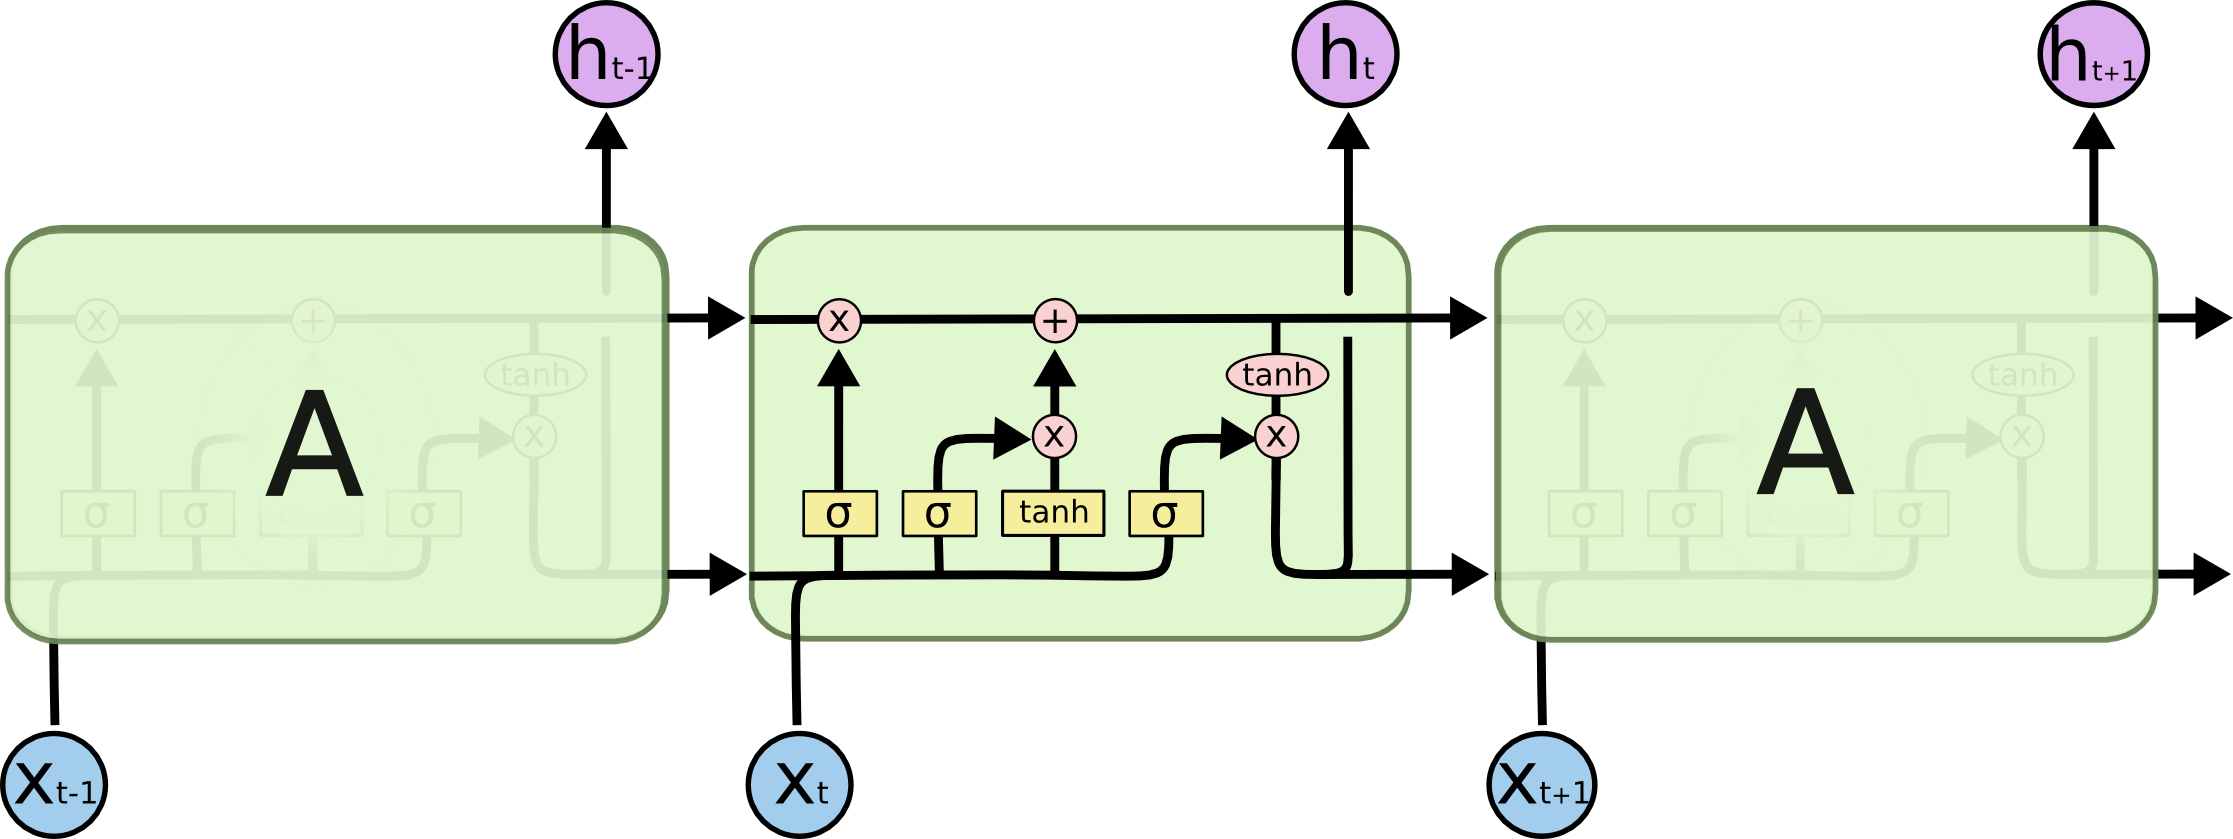
\includegraphics[width=0.90\textwidth]{img/lstm_colah.png}
	\caption{Schemat komórki LSTM.\\ Źródło: http://colah.github.io/posts/2015-08-Understanding-LSTMs/}
	\label{fig:lstm}
\end{figure}

LSTM jest jedną z popularniejszych architektur RNN. Hochreiter i Schmidhuber zaproponowali architekturę Long Short-Term Memory (LSTM) \cite{LSTM} w 1997. Zwykła sieć RNN składa się jedynie ze stanu sieci $h$, oraz wejścia $x$, które są wejściem warstwy ukrytej sieci. Wyjście warstwy ukrytej jest wyjściem sieci. Struktura komórki LSTM jest bardziej skomplikowana i składa się z wektora stanu sieci $h$, komórki pamięci $C$, oraz czterech ukrytych warstw sieci. Schemat ze strukturą sieci został przedstawiony na rys. \ref{fig:lstm}.

Warstwy sieci LSTM z sigmoidalnymi funkcjami aktywacji są nazywane bramkami multiplikatywnymi. Sigmoidalna funkcja aktywacji jest opisywana za pomocą wzoru:

\begin{equation}
	\sigma(x) = \frac{1}{e^{-x} + 1}
\end{equation}

i posiada zbiór wartości $(0, 1)$. Przemnożenie wyjścia tej warstwy z dowolną wartością powoduje jej przeskalowanie, przez co warstwy te są wykorzystywane do kontrolowania wartości zmiennych komórki LSTM. Dodatkowo bramki jako warstwy sieci posiadają wagi, które ulegają modyfikacji w trakcie uczenia, przez co LSTM w procesie uczenia zyskują informację o tym kiedy i w jaki sposób uaktualnić swój stan i komórkę pamięci na podstawie obecnie posiadanych informacji. Wyróżnia się 3 bramki. Pierwszą z nich jest forget gate. Jest ona odpowiedzialna za zmniejszanie wartości aktualnie znajdującej się w komórce pamięci. Operacja realizowana przez forget gate jest opisywana wzorem: 

\begin{equation}
	f_t = \sigma( W_f [ h_{t-1}, x_t ] + b_f )
\end{equation}

Gdzie $W_f$ i $b_f$ to odpowiednio wagi i bias warstwy, $h_{t-1}$ to stan komórki z poprzedniego kroku, a $x_t$ to aktualne wejście sieci. Kolejną bramką jest input gate. Realizowana operacja wyraża się analogicznym wzorem:

\begin{equation}
	i_t = \sigma( W_i [ h_{t-1}, x_t ] + b_i )
\end{equation}

Intuicyjnie jest ona odpowiedzialna za określanie w jakim stopniu należy zaktualizować komórkę pamięci sieci na podstawie aktualnego wejścia sieci $x_t$ i stanu z poprzedniego kroku $h_{t-1}$. Na podstawie $x_t$ i $h_{t-1}$ jest obliczana wartość $\tilde{C}_t$:

\begin{equation}
	\tilde{C}_t = tanh( W_c [ h_{t-1}, x_t ] + b_C )
\end{equation}

Wartość $\tilde{C}_t$ może być określona jako kandydat do zastąpienia stanu komórki z poprzedniego kroku $C_{t-1}$. Aktualna wartość $C_t$ jest zatem obliczana ze wzoru:

\begin{equation}
	C_t = f_t \odot C_{t-1} + i_t \odot \tilde{C}_t
\end{equation}

gdzie $\odot$ oznacza iloczyn Hadamarda (iloczyn wszystkich elementów wektora lub macierzy). Ostatnią bramką jest output gate. Realizowana operacja jest dana wzorem:

\begin{equation}
	o_t = \sigma( W_o [ h_{t-1}, x_t ] + b_o )
\end{equation}

Służy do określania, sposobu w jaki zostanie zaktualizowany stan $h$ w aktualnym kroku $t$, co wyraża się równaniem:

\begin{equation}
	h_t = o_t \odot tanh( C_t )
\end{equation}

Warto zwrócić uwagę, że w powyższym równaniu nie występują wagi ani bias, więc $tanh$ nie jest utożsamiony z warstwą sieci neuronowej.



\section{GRU}

\begin{figure}
\centering
	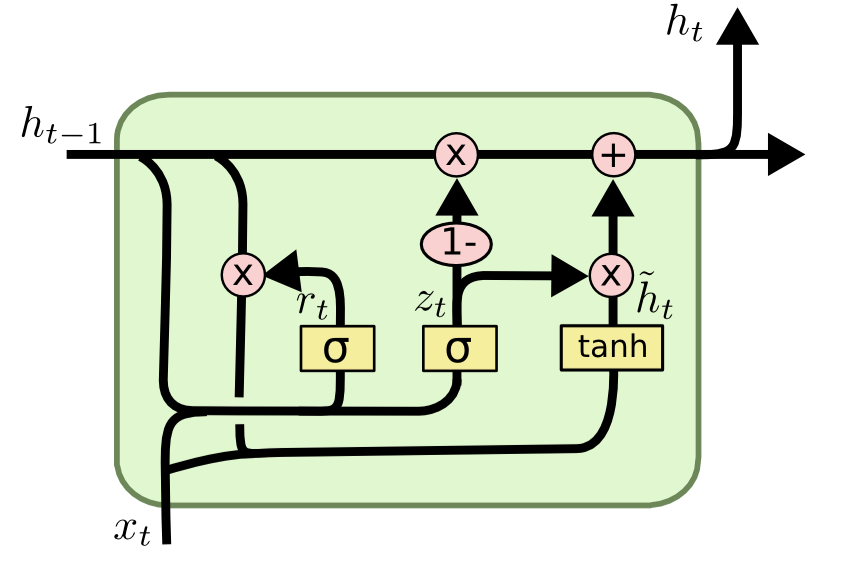
\includegraphics[width=0.5\textwidth]{img/LSTM3-var-GRU.png}
	\caption{Schemat komórki GRU.\\ Źródło: http://colah.github.io/posts/2015-08-Understanding-LSTMs/}
	\label{fig:gru}
\end{figure}

\chapter{Problem badawczy}

\section{ReNet}

\section{Proponowana architektura sieci}

\section{Krzywe wypełniające przestrzeń}




\chapter{Przeprowadzone badania}

\section{Metodyka badań}

\section{Opis eksperymentu}

\subsection{Zbiór danych}

\subsection{Wykorzystane narzędzia i hardware}

\subsection{Dobór hiperparametrów modelu}



\chapter{Wyniki}


\chapter{Wnioski}

\bibliography{bibliography}

\listoffigures

\end{document}